\documentclass{article}
\usepackage[utf8]{inputenc}

\documentclass[a4paper]{article}
\usepackage[12pt]{extsizes}
\usepackage{amsmath,amsthm,amssymb}
\usepackage[hidelinks]{hyperref} 
\usepackage[warn]{mathtext}
\usepackage[T1,T2A]{fontenc}
\usepackage[utf8]{inputenc}
\usepackage[english,russian]{babel}
\usepackage{tocloft}
\linespread{1.5}
\usepackage{indentfirst}
\usepackage{setspace}
%\полуторный интервал
\onehalfspacing

\newcommand{\RomanNumeralCaps}[1]
    {\MakeUppercase{\romannumeral #1}}

\usepackage{amssymb}

\usepackage{graphicx, float}
\graphicspath{{pictures/}}
\DeclareGraphicsExtensions{.pdf,.png,.jpg}
\usepackage[left=25mm,right=1cm,
    top=2cm,bottom=20mm,bindingoffset=0cm]{geometry}
\renewcommand{\cftsecleader}{\cftdotfill{\cftdotsep}}

\addto\captionsrussian{\renewcommand{\contentsname}{СОДЕРЖАНИЕ}}
\addto\captionsrussian{\renewcommand{\listfigurename}{СПИСОК ИЛЛЮСТРАЦИЙ}}

\usepackage{fancyhdr}
\usepackage[nottoc]{tocbibind}

\fancypagestyle{plain}{
\fancyhf{}
\renewcommand{\headrulewidth}{0pt}
\fancyhead[R]{\thepage}
}

\usepackage{blindtext}
\pagestyle{myheadings}
\usepackage{hyperref}

\begin{document}
\begin{titlepage}
  \begin{center}
    \large
    Санкт-Петербургский политехнический университет Петра Великого
    
    Институт прикладной математики и механики
    
    \textbf{Высшая школа прикладной математики и вычислительной физики}
    \vfill
    \textsc{\textbf{\Large{Отчёт по лабораторной работе №5}}}\\[5mm]
    \\ по дисциплине
    \\ <<Математическая статистика>>\\
\end{center}

\vfill

\begin{tabular}{l p{140} l}
Выполнила студентка \\группы 3630102/80401 && Мамаева Анастасия Сергеевна \\
\\
Проверил\\Доцент, к.ф.-м.н.& \hspace{0pt} &   Баженов Александр Николаевич \\\\
\end{tabular}

\hfill \break
\hfill \break
\begin{center} Санкт-Петербург \\2021 \end{center}
\thispagestyle{empty}
\end{titlepage}
\newpage
\newpage
\begin{center}
    \setcounter{page}{2}
    \tableofcontents
\end{center}
\newpage
\begin{center}
    \setcounter{page}{3}
    \listoffigures
\end{center}

\newpage

\section {Постановка задачи}
\noindent Сгенерировать двумерные выборки размерами 20, 60, 100 для нормального двумерного распределения $N(x,y,0,0,1,1,\rho)$. Коэффициент корреляции $\rho$ взять равным 0, 0.5, 0.9. Каждая выборка генерируется 1000 раз и для неё вычисляются: среднее значение, среднее значение квадрата и дисперсия коэффициентов корреляции Пирсона, Спирмена и квадрантного коэффициента корреляции. Повторить все вычисления для смеси нормальных распределений:
\begin{equation}
	f(x,y) = 0.9N(x,y,0,0,1,1,0.9) + 0.1N(x,y,0,0,10,10,-0.9)
\end{equation}
\noindent Изобразить сгенерированные точки на плоскости и нарисовать эллипс равновероятности.

\section{Теория}
\subsection{Двумерное нормальное распределение}
\noindent Двумерная случайная величина $(X,Y)$ называется распределённой нормально (или просто нормальной), если её плотность вероятности определена формулой
\begin{equation}
N(x, y, \bar{x}, \bar{y}, \sigma_{x}, \sigma_{y}, \rho) = 
\frac{1}{2\pi\sigma_{x}\sigma_{y}\sqrt{1-\rho^{2}}} \times
exp{\begin{Bmatrix}
	-\frac{1}{2(1-\rho^{2})}
	\begin{bmatrix}
	\frac{(x-\bar{x})^{2}}{\sigma_{x}^{2}} - 2\rho\frac{(x-\bar{x})(y-\bar{y})}{\sigma_{x}\sigma_{y}} + \frac{(y-\bar{y})^{2}}{\sigma_{y}^{2}}
	\end{bmatrix}
	\end{Bmatrix}}
\end{equation}
Компоненты $X,Y$ двумерной нормальной случайной величины также распределены нормально с математическими ожиданиями $\bar{x}$,$\bar{y}$ и средними квадратическими отклонениями $\sigma_{x},\sigma_{y}$ соответственно [1, с. 133-134].
Параметр $\rho$ называется коэффициентом корреляции.


\subsection{Корреляционный момент (ковариация) и коэффициент корреляции}
\noindent Корреляционным моментом, иначе ковариацией, двух случайных величин X и Y называется математическое ожидание произведения отклонений этих случайных величин от их математических ожиданий [1, с. 141].
\begin{equation}
K = cov(X, Y) = M[(X - \bar{x})(Y - \bar{y})]
\label{K}
\end{equation}
Коэффициентом корреляции $\rho$ двух случайных величин X и Y называется отношение их корреляционного момента к произведению их средних квадратических отклонений:
\begin{equation}
\rho = \frac{K}{\sigma_{x}\sigma_{y}}
\label{ro}
\end{equation}
Коэффициент корреляции — это нормированная числовая характеристика, являющаяся мерой близости зависимости между случайными величинами к линейной [1, с. 150].

\subsection{Выборочные коэффициенты корреляции}
\subsubsection{Выборочный коэффициент корреляции Пирсона}
\noindent Пусть по выборке значений ${x_{i},y_{i}}^{n}_{1}$ двумерной с.в. (X,Y ) требуется оценить коэффициент корреляции $\rho = \frac{cov(X,Y)}{\sqrt{DXDY}}$ . Естественной оценкой для $\rho$ служит его статистический аналог в виде выборочного коэффициента корреляции, предложенного К.Пирсоном, —
\begin{equation}
r = \frac{
	\frac{1}{n}\sum{(x_{i} - \bar{x})(y_{i}-\bar{y})}
}{
	\sqrt{\frac{1}{n}\sum{(x_{i} - \bar{x})^{2}}\frac{1}{n}\sum{(y_{i} - \bar{y})^{2}}}
}=\frac{K}{s_{X}s_{Y}},
\label{r}
\end{equation}
где $K,s^{2}_{X},s^{2}_{Y}$ — выборочные ковариация и дисперсии с.в. X и Y [1, c. 535].


\subsubsection{Выборочный квадрантный коэффициент корреляции}
\noindent Кроме выборочного коэффициента корреляции Пирсона, существуют и другие оценки степени взаимосвязи между случайными величинами. К ним относится выборочный квадрантный коэффициент корреляции
\begin{equation}
r_{Q} = \frac{(n_{1} + n_{3}) - (n_{2} + n_{4})}{n},
\label{rQ}
\end{equation}

\noindent где $n_1, n_2, n_3, n_4 - $ количества точек с координатами $x_i, y_i$, попавшими соответственно в I, II, III, IV квадранты декартовой системы с осями $x'=x-med x$, $y'=y-med y$ и с центром в точке с координатами $(med x, med y)$



\subsubsection{Выборочный коэффициент ранговой корреляции Спирмена}
\noindent На практике нередко требуется оценить степень взаимодействия между качественными признаками изучаемого объекта. Качественным называется признак, который нельзя измерить точно, но который позволяет сравнивать изучаемые объекты между собой и располагать их в порядке убывания или возрастания их качества. Для этого объекты выстраиваются в определённом порядке в соответствии с рассматриваемым признаком. Процесс упорядочения называется ранжированием, и каждому члену упорядоченной последовательности объектов присваивается ранг, или порядковый номер. Например, объекту с наименьшим значением признака присваивается ранг 1, следующему за ним объекту — ранг 2, и т.д. Таким образом, происходит сравнение каждого объекта со всеми объектами изучаемой выборки.
\newline
Если объект обладает не одним, а двумя качественными признаками — переменными X и Y , то для исследования их взаимосвязи используют выборочный коэффициент корреляции между двумя последовательностями рангов этих признаков.
\newline
Обозначим ранги, соотвествующие значениям переменной X, через u, а ранги, соотвествующие значениям переменной Y, — через v.
\newline
Выборочный коэффициент ранговой корреляции Спирмена определяется как выборочный коэффициент корреляции Пирсона между рангами u,v переменных X,Y :
\begin{equation}
r_{S} = \frac{
	\frac{1}{n}\sum{(u_{i} - \bar{u})(v_{i}-\bar{v})}
}{
	\sqrt{\frac{1}{n}\sum{(u_{i} - \bar{u})^{2}}\frac{1}{n}\sum{(v_{i} - \bar{v})^{2}}}
},
\label{rS}
\end{equation}
где $\bar{u} = \bar{v} = \frac{1 + 2 + ... + n}{n} = \frac{n + 1}{2}$ — среднее значение рангов [1, с. 540-541].


\subsection{Эллипсы рассеивания}
\noindent Рассмотрим поверхность распределения, изображающую функцию (1). Она имеет вид холма, вершина которого находится над точкой $(\bar{x},\bar{y})$.
\newline
В сечении поверхности распределения плоскостями, параллельными оси $ N(x, y, \bar{x}, \bar{y}, \sigma_{x}, \sigma_{y}, \rho)$, получаются кривые, подобные нормальным кривым распределения. В сечении поверхности распределения плоскостями, параллельными плоскости xOy, получаются эллипсы. Напишем уравнение проекции такого эллипса на плоскость xOy: 
\begin{equation}
\frac{(x-\bar{x})^{2}}{\sigma_{x}^{2}} - 
2\rho\frac{(x-\bar{x})(y-\bar{y})}{\sigma_{x}\sigma_{y}}+
\frac{(y-\bar{y})^{2}}{\sigma_{y}^{2}} = const
\label{ellipse}
\end{equation}
Уравнение эллипса \ref{ellipse} можно проанализировать обычными методами аналитической геометрии. Применяя их, убеждаемся, что центр эллипса \ref{ellipse} находится в точке с координатами $(\bar{x},\bar{y})$; что касается направления осей симметрии эллипса, то они составляют с осью Ox углы, определяемые уравнением
\begin{equation}
tg(2\alpha) = \frac{2\rho\sigma_{x}\sigma_{y}}{\sigma_{x}^{2} - \sigma_{y}^{2}}
\label{angle}
\end{equation}
Это уравнение дает два значения углов: $\alpha$ и $\alpha_{1}$, различающиеся на $\frac{\pi}{2}$.
\newline
Таким образом, ориентация эллипса \ref{ellipse} относительно координатных осей находится в прямой зависимости от коэффициента корреляции $\rho$ системы (X,Y); если величины не коррелированны (т.е. в данном случае и независимы), то оси симметрии эллипса параллельны координатным осям; в противном случае они составляют с координатными осями некоторый угол.
\newline
Пересекая поверхность распределения плоскостями, параллельными плоскости xOy, и проектируя сечения на плоскость xOy мы получим целое семейство подобных и одинаково расположенных эллипсов с общим центром $(\bar{x},\bar{y})$. Во всех точках каждого из таких эллипсов плотность распределения $ N(x, y, \bar{x}, \bar{y}, \sigma_{x}, \sigma_{y}, \rho)$ постоянна. Поэтому такие эллипсы называются эллипсами равной плотности или, короче эллипсами рассеивания. Общие оси всех эллипсов рассеивания называются главными осями рассеивания [2, с. 193-194].

\section{Программная реализация}
\noindent Лабораторная работа выполнена на языке Python вресии 3.7 в среде разработки JupyterLab. Использовались дополнительные библиотеки:
 \begin{enumerate}
        \item scipy (генерация выборок)
        \item statsmodels, statistics (построение эмпирических функций распределения)
        \item matplotlib (визуализация)
        \item numpy (вычисление ряда числовых характеристик)
    \end{enumerate}
В приложении находится ссылка на GitHub репозиторий с исходныи кодом.

\section{Результаты}
\subsection{Выборочные коэффициенты корреляции}
	\begin{table}[H]
		\centering
		\begin{tabular}{| c | c | c | c |}
			
			\hline
			$\rho=0$  & $r$      & $r_S$  & $r_Q$ \\
			\hline
            $E(z)$    & -0.014 & -0.021 & 0.0   \\
            $E(z^{2})$  & 0.028  & 0.029  & 0.04  \\
            $D(z)$    & 0.055  & 0.056  & 0.056 \\
			\hline
			$\rho=0.5$ & $r$      & $r_S$  & $r_Q$ \\
			\hline
			$E(z)$      & 0.509 & 0.474 & 0.4   \\
            $E(z^{2})$   & 0.26  & 0.224 & 0.16  \\
            $D(z)$     & 0.032 & 0.036 & 0.046 \\
			\hline
			$\rho=0.9$  & $r$      & $r_S$  & $r_Q$ \\
			\hline
			$E(z)$      & 0.905 & 0.88  & 0.8   \\
            $E(z^{2})$    & 0.818 & 0.774 & 0.64  \\
            $D(z)$      & 0.002 & 0.004 & 0.028 \\
			\hline
			
		\end{tabular}{}
		\caption{Двумерное нормальное распределение, n = 20}
		\label{tab:n20}
	\end{table}
	
	
	\begin{table}[H]
		\centering
		\begin{tabular}{| c | c | c | c |}
			
			\hline
			$\rho = 0$ & $r$      & $r_S$  & $r_Q$ \\
			\hline
			$E(z)$    & 0.005 & 0.005 & 0.0   \\
            $E(z^{2})$  & 0.008 & 0.008 & 0.004 \\
            $D(z)$    & 0.018 & 0.018 & 0.018 \\
			\hline
			$\rho = 0.5$ & $r$      & $r_S$  & $r_Q$ \\
			\hline
			$E(z)$      & 0.498 & 0.484 & 0.333 \\
            $E(z^{2})$    & 0.248 & 0.234 & 0.111 \\
            $D(z)$      & 0.009 & 0.01  & 0.015 \\
			\hline
			$\rho = 0.9$ & $r$      & $r_S$  & $r_Q$ \\
			\hline
			$E(z)$      & 0.901 & 0.886 & 0.733 \\
            $E(z^{2})$    & 0.811 & 0.785 & 0.538 \\
            $D(z)$      & 0.001 & 0.001 & 0.008 \\
			\hline
			
		\end{tabular}{}
		\caption{Двумерное нормальное распределение, n = 60}
		\label{tab:n60}
	\end{table}
	
	
	
	\begin{table}[H]
		\centering
		\begin{tabular}{| c | c | c | c |}
			
			\hline
			$\rho = 0$ & $r$      & $r_S$  & $r_Q$ \\
			\hline
			$E(z)$    & 0.003 & 0.002 & 0.0   \\
            $E(z^{2})$  & 0.005 & 0.005 & 0.006 \\
            $D(z)$    & 0.01  & 0.01  & 0.011 \\
			\hline
			$\rho = 0.5$ & $r$      & $r_S$  & $r_Q$ \\
			\hline
			$E(z)$      & 0.503 & 0.484 & 0.32  \\
            $E(z^{2})$    & 0.253 & 0.234 & 0.102 \\
            $D(z)$      & 0.006 & 0.007 & 0.009 \\
			\hline
			$\rho = 0.9$ & $r$      & $r_S$  & $r_Q$ \\
			\hline
			$E(z)$      & 0.9   & 0.889 & 0.72  \\
            $E(z^{2})$    & 0.811 & 0.79  & 0.518 \\
            $D(z)$      & 0.0   & 0.001 & 0.005 \\
			\hline
			
		\end{tabular}{}
		\caption{Двумерное нормальное распределение, n = 100}
		\label{tab:n100}
	\end{table}
	
	
	\begin{table}[H]
		\centering
		\begin{tabular}{| c | c | c | c |}
			
			\hline
			$size = 20$ & $r$      & $r_{S}$ & $r_{Q}$ \\
			\hline
			$E(z)$      & 0.8   & 0.88  & 0.6   \\
            $E(z^{2})$    & 0.64  & 0.774 & 0.36  \\
            $D(z)$      & 0.009 & 0.004 & 0.035 \\
			\hline
			$size = 60$ & $r$      & $r_{S}$ & $r_{Q}$ \\
			\hline
			$E(z)$      & 0.794 & 0.886 & 0.6   \\
            $E(z^{2})$    & 0.631 & 0.785 & 0.36  \\
            $D(z)$      & 0.003 & 0.001 & 0.011 \\
			\hline
			$size = 100$ & $r$      & $r_{S}$ & $r_{Q}$ \\
			\hline
			$E(z)$       & 0.791 & 0.889 & 0.6   \\
            $E(z^{2})$     & 0.626 & 0.79  & 0.36  \\
            $D(z)$       & 0.001 & 0.001 & 0.007 \\
			\hline
			
		\end{tabular}{}
		\caption{Смесь нормальных распределений}
		\label{tab:mix_normal}
	\end{table}
	
\subsection{Эллипсы рассеивания}
	
	\begin{figure}[H]
		\centering
		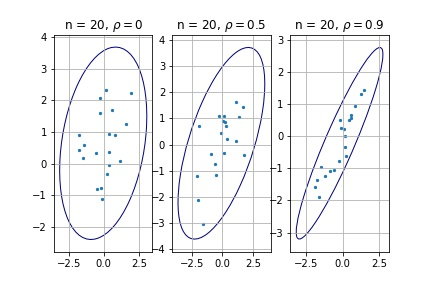
\includegraphics[width = 13cm, height = 8cm]{n20.jpg}
		\caption{Двумерное нормальное распределение, n = 20}
		\label{fig:n20}
	\end{figure}
	
	\begin{figure}[H]
		\centering
		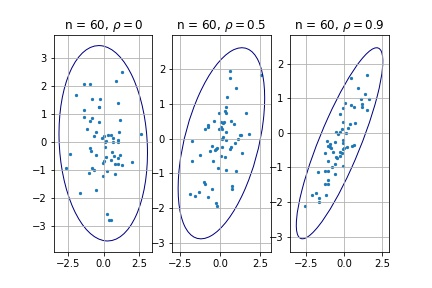
\includegraphics[width = 13cm, height = 8cm]{n60.jpg}
		\caption{Двумерное нормальное распределение, n = 60}
		\label{fig:n60}
	\end{figure}

	\begin{figure}[H]
		\centering
		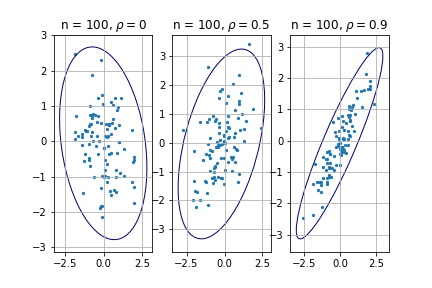
\includegraphics[width = 13cm, height = 8cm]{n100.jpg}
		\caption{Двумерное нормальное распределение, n = 100}
		\label{fig:n100}
	\end{figure}

\section{Обсуждение}
\subsection{Ядерные оценки плотности распределения}
\noindent Для двумерного нормального распределения дисперсии выборочных коэффициентов корреляции упорядочены следующим образом: $r < r_{S} < r_{Q}$; для смеси распределений получили обратную картину: $r_{Q} < r_{S} < r$.
\newline
\noindent Процент попавших элементов выборки в эллипс рассеивания (95$\%$-ная доверительная область) примерно равен его теоретическому значению (95$\%$).

\section{Приложение}
\noindent Код программы GitHub URL:\\
\newline https://github.com/Brightest-Sunshine/Math-Statistic-2021/blob/main/Lab5/Lab5.ipynb
\end{document}
